% -*- TeX -*- -*- UK -*- -*- Soft -*-

\chapter{Visualizing Neural Nets}
\label{sec:VisualizingNeuralNets}

Prepared by CJ Willers.


\section{Overview}
\label{sec:OverviewAppc}

This document reports on analysis and experimental work to better understand neural nets, by visualizing the building blocks separately.  It is shown that a single neuron provides the same capability as a simple linear classifier; that is, to separate a data set into two classes, based on a linear discrimination surface (a line in the two-dimensional plane).  The mathematical shape of  the non-linear output of a solitary neuron is of little practical significance.

The almost magical power of neurons only really come to fruition when the neurons are connected in a network, when: 
\begin{enumerate}
\item more than one layer of neurons are used, 
\item the outputs of the neurons are limited in a non-linear manner, and 
\item the weights of all neurons in the network can be adjusted to optimise performance.
\end{enumerate}

When layers of non-linear neurons are used, the simple linear discrimination capability of a single neuron can be applied to define complex discrimination curves.  These complex curves are constructed of smaller sections of the individual neuron discrimination lines.

\section{A Single Neuron}

The artificial neuron is the core computing element, simulating a biological neuron.  The artificial neuron receives a number of signals (small voltages) of arbitrary (analogue) value from other artificial neurons.  The artificial neuron then weights (multiplies by a set of values) the input signals, adds them together.  The sum is then distorted by a non-linear process, to yield the output signal. The output signal is then fed into neurons in the network.   The artificial neuron is modelled in mathematical form as follows:

\begin{figure}[tb]
\centering
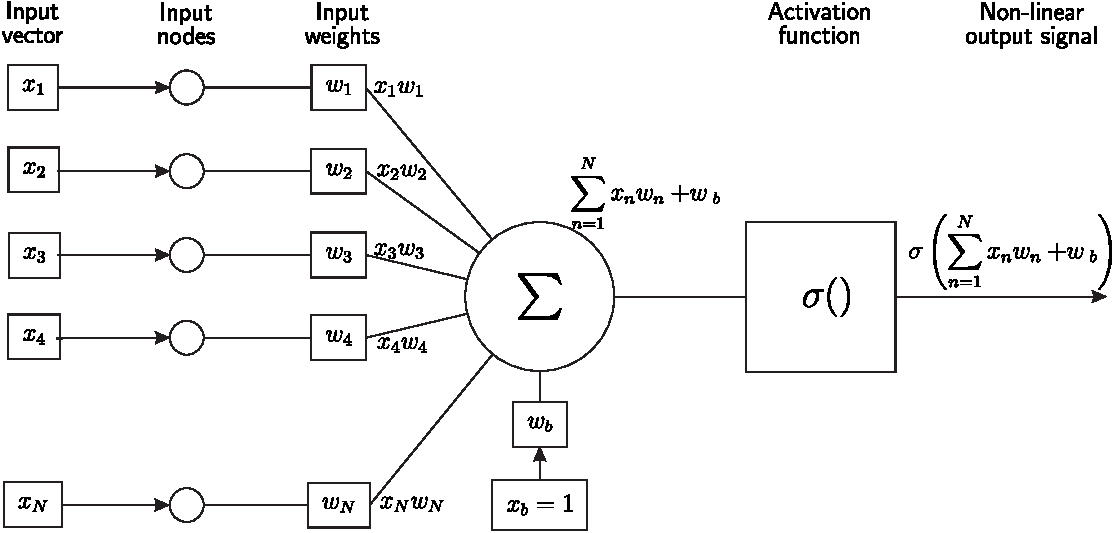
\includegraphics[width=\textwidth]{eps/neuralnetconcept}
\caption{Neural net concept\label{fig:neuralnetconcept}}
\end{figure}

Consider a very simple neuron with only two inputs $(x_1,x_2)$.  Then $\bm{x}=(x_1,x_2)$  and  $\bm{w}=(w_1,w_2)$, and the artificial neuron operation is $y = \varphi(\bm{x}\cdot\bm{w}+w_b)$, where $\varphi$  is any non-linear function and  $w_b$ is the neuron's bias weight.  Compare the mathematical expression of a two-input neural net with a simple straight line in a two-dimensional Cartesian space:

Neural net: $z=\varphi(w_1x_1+w_2x_2+b)$

Straight line:  $0=(mx+(-1)y+c)$

Note the remarkable resemblance between the two equations.  Suppose, for a short while, that the non-linear function can be 'forced' to be linear (in other words, the $\varphi()$ function   disappears).  Also consider the neuron when $z=0$.  Then the equation for the straight line and the (assumed simplified neuron) have the same form.  Under these two conditions, one can state: $w_1=m$, $w_2=-1$, $x_1=x$, $x_2=y$, $b=c$.  It is evident that the two weights and bias of a two-input neuron defines a straight line.  Returning to fix the two simplifying assumptions, we note that the straight line now describes the locus (line) where the non-linear function $\varphi()$ is zero.  

Suppose that the non-linear function is the tansig function\cite{stackexchangeEllefsen2015,WikiPediaHyperbolicfunction2019,NickBecker2017}, 
\begin{equation}
\varphi(x)
=\left(\frac{2}{1+e^{-bx}}\right)-1
=\left(\frac{1-e^{-bx}}{1+e^{-bx}}\right)
\end{equation}  
where, normally, $b=2$ for the $\tanh(x)$ function.
The derivative of the tansig function is 
\begin{equation}
 \varphi^\prime(x)
 = \frac{b}{2} \left(1+\varphi(x))(1-\varphi(x)\right)
 = \frac{b}{2}\left(1-\varphi^2(x)\right)
\end{equation}


Imagine a sheet of paper formed into a two-dimensional tansig shape (see figures on the left).  Visualize walking along the $z=0$ contour of the tansig surface.  As we walk along this line, to the left of us, the tansig surface falls away to $-1$, while on the right hand side, the tansig surface rises to $+1$.  Note, however, that the tansig $z=0$ line is the equation of the straight line derived from the neuron equation, $0=z=\varphi(w_1x_1+w_2x_2+b)$ , since $\varphi(x)=0$.  The neuron's weights and bias therefore determines the exact location and direction of the tansig surface in the two-dimensional Cartesian space.  

Note that while $\varphi(w_1x_1+w_2x_2+b)$  and  $\varphi(2w_1x_1+2w_2x_2+2b)$ both result in the same straight line in the two-dimensional plane, they yield two very different surfaces.  The slope of the surface, away from the  $\varphi(x)=0$ line, is strongly affected by the neuron's weights and bias.  

\section{Linear Classifiers and Neurons}

\begin{figure}[tb]
\centering
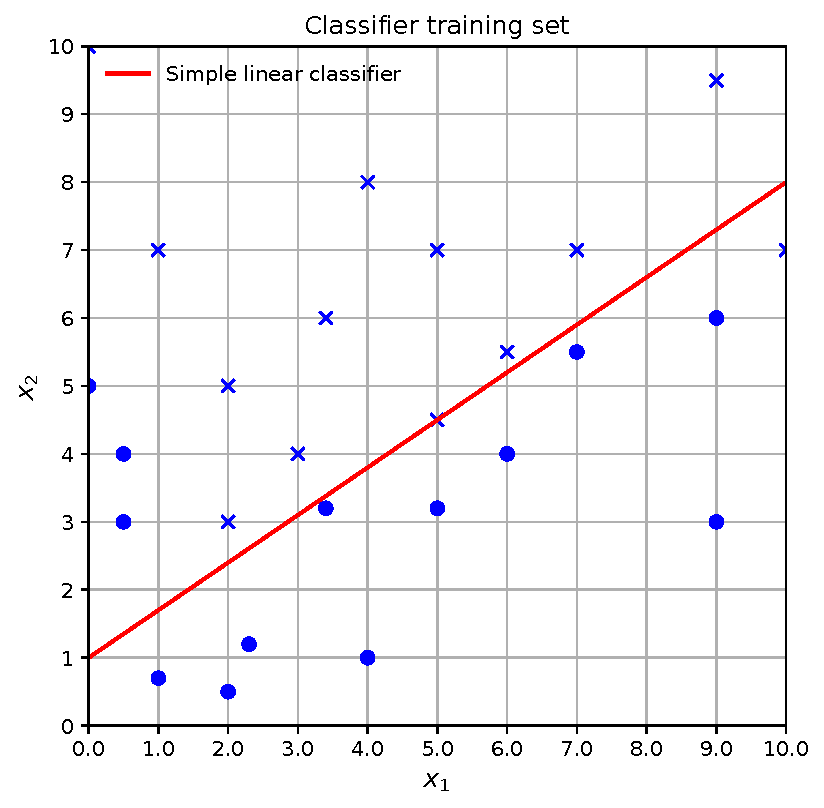
\includegraphics[width=.6\textwidth]{pic/chC-trainingset}
\caption{Neural net concept\label{fig:chC-trainingset}}
\end{figure}

Figure~\ref{fig:chC-trainingset} shows data from two classes plotted in terms of feature $x_1$ and feature $x_2$.  Objects from class O are marked with a circle, and objects from class * are marked with an asterisk.  

The task at hand is to determine a method to discriminate between the two classes O and * on the basis of the feature sets $x_1$ and $x_2$.  While it is easy to do this by visual observation, the objective is to determine an accurate and robust mathematical means to perform this task.  

As a first attempt, draw a straight line as shown in the figure above.  This line is a simple linear (straight line) classifier, where the line $y=\frac{10}{7}(x-1)$  represents the classification boundary.  All objects with features 'above' the line belongs to class O, while the object with features 'below' the line belongs to class *.  Observing the figure carefully, one notices that not all the class O-objects fall 'above' the line.  There are also some class * objects above the line.   In other words, the two classes denoted by * and O cannot be discriminated by this simple discriminator.  

As a second attempt, combine the linear classifier shown above with the tansig surface shown on the previous page.  This is done by orienting the tansig surface along the straight line defined by the linear classifier.  This seemingly simple operation has significant implications.  It now becomes clear that a two-dimensional \textit{(two-input) neuron is a linear discrimination element}, with a non-linear output function.    It is very important to observe that this two-input neuron defines a single, straight line between two classes, and that this has nothing to do with the non-linear output function - the discrimination ability of the single neuron is determined solely by its weights and bias.  Sadly, still, this single neuron has the same limitation as linear discriminator. 

Suppose we can add more straight lines (neurons), and somehow define in which regions they should operate --- then we can define a complex discrimination line as a set of shorter segments.  Enter neural networks.

\section{Neural networks}

Adding more discrimination lines is easy: just add more input neurons.  If we need 5 segments to define the discrimination line in the two-dimensional plane, use 5 neurons.   Note that, in effect, we are using 5 linear classifiers (straight lines), but we have to limit the operating range of each classifier to a small segment of its total length.    In effect, this means that all the straight lines are optimised to achieve the best discrimination, but each in his own (local) area.  This is where the hidden layer(s) come to the rescue:  each first-layer neuron's output is scaled by the weight where this neuron feeds into the second layer, thereby 'activating' only selected sections of each of the linear classifiers.  Note, however, that the optimisation is not done separately for each line - all elements in the net are trained as a whole, with full consideration of the interaction and dependencies between elements.  

To illustrate these concepts, a small neural net was trained to discriminate between the O and * classes.  Five hidden layer neurons and one output neuron were used.  There are only two inputs $(x_1,x_2)$ , feeding into the hidden layer neurons.  When the net is trained, the weights and bias values are adjusted to find an optimum discrimination.  Class * object provide an output signal of $+1$, while a Class O object provides a $-1$ output signal.  

In our journey through neural network land,  we start of by considering each neuron on its own, then the neural net is assembled by adding the hidden layer neurons one by one, until we reach the final network.    The three-dimensional graphs shown on the following pages represent the output of the neuron (or network), for all possible input values  $(x_1,x_2)$  with $0\leq x_1 \leq 10$  and  $0\leq x_2 \leq 10$.  The graphs were obtained by defining a two-dimensional grid with grid interval of 0.25.  For each of the 40$\times$40  $(x_1,x_2)$ points, the neuron/network responses were calculated and plotted in the three-dimensional graph format.   We can see how the neuron (or network) will respond to all possible input signal combinations.   By careful study of these input-output graphs, the inner workings of the neural net becomes clear.

First, we will study the tansig surface shape of each neuron hidden neuron, and show how these hidden neurons each contribute a portion to the overall discrimination line.  Note that not all neurons seem to have the same dramatic effect, but keep in mind that the next layer can scale up this output when adding it to the other neuron signals.  In fact, the key to the neural network calculation is the fact that the outputs from these hidden layer neurons must be added in exactly the correct proportions to achieve the final discrimination objective.  

In experimenting with the net, it was quite interesting to observe how much the net behaviour changes, for just one small adjustment in the training set.  Even when using the same input data, different runs resulted in dramatically different shapes, just because of random differences in starting weights and biases.  The results shown here, therefore only demonstrate one possible solution, there are many other (equally valid) solutions.  These other solutions are obtained by repeated training, each time with different seeds to the random number generator. 

 
This graphs below show the individual responses of the hidden neurons.   Note that each of the neurons only provide a straight line, nothing more.   The lines are also widely different in slope and offset.  The outputs of these nets are also contained between $-1$ and $+1$, by the tansig function.   

The graph on the bottom right left shows the $y=mx+c$ lines for each of the hidden neurons.  Each line in this graph can be traced to the two dimensional shapes, since these lines trace out the $z=0$  for the tansig surfaces.  Note how each of the lines attempt to provide a measure of discrimination between the O and * classes.  None of these lines are able to provide the required separation between O and * classes.   

 
 
The graphs below show the sum of the neuron signals, starting with the bias, and then adding an additional neuron until all neuron signals are included.  The signals shown here are already scaled by the output neuron weights, in the correct proportions, but the non-linear output compression is not yet applied. 

Note how the output neuron weights (sign and magnitude) manipulate the signals from each of the previous layer neurons to build a surface that will eventually form the discrimination surface.  In particular, note how the class * area is growing in a positive direction, while the class O area is growing towards $-10$.  Keep in mind that the class * output must be $+1$ while the class O output must be $-1$.  As the neuron signals are added, the emerging shape approaches the required discrimination class regions 
 
 
The output signal from the output neuron (but before non-linear compression) net is shown below.   It is quite informative to study the graph and to identify the individual linear discrimination lines, and to observe how these lines are cleverly segmented by adding the neurons' signals together.   It is also evident that the hidden neuron signals  were scaled differently by the input weights on the output neuron.  

The key observation is that the hidden neuron outputs are limited by the tansig signal, and hence, their output values can be scaled \textit{differently} by the weights in the output layer.  If the hidden layer outputs were not limited, the output signals would be monotonically increasing/decreasing away from the $\varphi(0)=0$  line, and there would be little value in adding these increasing values together. 

This output response is the result of a happy dance of 15 weights, and 6 bias values, for the full range of input feature values.  Note that this net's output signal can vary from $-20$ to $+20$, depending on the input  $(x_1,x_2)$.    The distinctly visible plateaus are remnants from the tansig shapes of the input neurons.  

Since we are only interested in classifying between class O and class *, we define a threshold value of $0$, and compare the net output against this threshold to classify an object. 
\begin{enumerate}
\item where the net output is greater than zero is class * domain, and 
\item where the net output is less than zero is class O domain.  
\end{enumerate} 
the final shaping of the discrimination curve is shown on the left.  The two top graphs show the final output of the neural net before and after non-linear compression.  

The second graph shows the output of the neural net after the non-linear limiting in the output neuron.  Notice how effectively all the plateaus and valleys are removed, leaving only the discrimination curve.  Note, also the input neurons' straight line classification segments.

The third curve shows a plan or top view of the two-dimensional Cartesian space.   The original input values are shown, together with the neural net response, shown in a contour plot.  A contour plot shows constant value lines (exactly like contour lines on a map shown altitude).  The $z=0$  line is somewhere in the turquoise colour band (near the middle of the band).  

Everything to the left (blue) side of $z=0$  is class O,  while the space to the right (red) side of $z=0$  is class *.  Observe how effectively the net employs the 5 linear discriminators to build the complex discrimination shape.  

We can only visualize curves like these up to the third dimension, but it some means of visualization for higher dimensions are available, it could be a useful tool to confirm the net design.

\section{Alternative Perspective}

This chapter provides compelling evidence to consider an artificial  neural net as a cascaded collection of linear discrimination building lines, planes or hyperplanes.  The graphs clearly show a number of lines and various plateaus and valleys that meet our intuitive notion of 'discrimination'.

Note, however, that neither the neural net, nor the back-propagation algorithm has any conscious knowledge of any such discrimination lines of surfaces.  In the same sense that a falling rock has no knowledge of Newton's laws, the net performs its function without being bound by our own poorly construed mental pictures of how things work.

An alternative view on the operation of the neural net, which is just as valid as the above view, it to consider the neural net as a very large (but conceptually simple) mathematical equation.  This equation is formed by a large number of sub-equations (neurons).  The end effect is a black box (the equation) that has a number of inputs and a number of outputs.  Inside this black box, are the equation itself, plus a large number of parameters (weights and biases) that must be adjusted to the problem at hand.  In terms of our two dimensional problem, this is the same as fitting a $y=mx+c$ curve to a number of data points: the slope $m$ and offset $c$ are parameters that must be adjusted to minimize the curve-fit error.  

In our little experiment above, the training of the neural net meant finding the best set of  linear discriminators.  However, in terms of the black box model, training the net means finding the set of parameters (weights and biases) that minimizes the output error for the given training set.  The output error is defined as the mean error from the ideal output, for all the neurons, taken collectively.  This error is normally defined as the mean value of the square of all the errors from all the neurons
\begin{equation}
e = \frac{1}{N}\sum^N_{n=1}(o_n-t_n)^2
\end{equation}
where $e$  is the mean squared error,  $N$  is the number of test vectors in the training set,  $o$  is the observed neural net output signal, and $t$  is the target or true value in the training data.  The purpose with the training process is to minimize $e$  by finding the best set of weights and biases.  

Seen as a black box, with adjustable parameters, it becomes imperative that optimal parameter estimation procedures be found.  The neural network fraternity has done much work in developing algorithms and tools in this regard.  Large numbers of optimisation algorithms have been developed for the variety of network topologies.  The simple feed forward topology considered here is only one example of the larger set of neural networks.

The black box model simply says that the underlying mathematical equation is used as the basis and the best parameters must be found to fit the data.  Once these parameters are known, the black box will perform according to these parameters.  The training procedure therefore strives to find the best fit parameters, relative to the training data set.  The fact that this is a neural network, is only of consideration to derive the underlying mathematical equation, it is of no consequence once the equation has been finalized.  

\section{Conclusion}

This study only covers two-dimensional space, where the discrimination boundary is a straight line.  In three-dimensional feature space (three inputs), the boundary is a plane, where the plane's location and orientation is defined by the three weights and the bias.  In higher order dimensions, the discrimination boundaries become hyper-planes.  Even though visualization becomes difficult, the fundamental principle still remains as outlined in this document for two dimensions.

The weights of the first layer neurons define the linear discriminators, while the weights in subsequent layers manipulates the linear discriminators so that only the required segments are effective.  On a meta level, one can say that the next layer weights perform linear discrimination on the outputs of the previous layer neurons.  This effect of abstract levels of next layers manipulating previous layers becomes hard to visualize.

It is generally accepted that the human brain has neuron connectivity of the order \num{10e4} (see \cite{WikiPediaNeuron2019}), this means that the brain can assemble discrimination hyper-surfaces in \num{10e4}  dimensional space.  Furthermore, the brain's complex feedback paths and ability to have thousands of 'hidden layers' hints that the brain can form discrimination surfaces of almost unlimited complexity.  Our work with small networks are but feeble attempts in comparison with the complexity of natural neural networks.  


Matlab code used to create the graphs in this paper
\begin{lstlisting}

% simnn.m

% some graphics stuff
set(0,'Units','pixels');
scnsize=get(0,'Screensize');


pt=[2   5
    3   4
    10   7
    1   7
    3.4 6.0
    7   7
    0  10
    6   5.5
    9   9.5
    5   7
    4   8
    2   3
    5   4.5  % last of first set   
    1   .7
    0.5 3
    5   3.2
    0.5 4
    3.4 3.2
    2.3 1.2
    7   5.5
    6   4
    9   6
    4   1
    2   0.5 
    0 5 
    9   3    
    ];
    
p=pt';
t=[ones(1, 13) -1*ones(1, 13)];

trainnnet=0;
if (trainnnet==1)
% train this net
    figure(1)
    net=newff([0 10 ; 0 10  ],[5 1], {'tansig','tansig'}, 'trainlm');
    net.trainParam.show = 5;
    net.trainParam.epochs = 100;
    net.trainParam.goal = 1e-5;
    net=train(net,p,t);
else
    load visual
end 



% here we evaluate the net's performance against the training set
a=sim(net,p);

tt=[1:size(a,2)];
z=0*ones(size(tt));

figure(2)

plot(tt,t,tt,z,tt,a)
title('testing net output vs target')

disp('training set results')
legal=(a>0);
nonlegal=(a<=0);

corleg=sum(legal(1:13))/13
errleg=1-corleg
cornon=sum(nonlegal(14:26))/13
errnon=1-cornon


x=[0:.25:10];
y=[0:.25:10];

xx=x'*ones(size(y));
yy=ones(size(x'))*y;
%mesh(xx)
%mesh(yy)

% layer 1, neuron 1
disp('net.IW{1,1}(1,2) to get the weight between neuron 1 and input 2:')
disp( 'net.b{1}(4) to get the bias in layer 1, neuron4:')

w111=net.IW{1,1}(1,1)
w112=net.IW{1,1}(1,2)
b11=net.b{1}(1);
z=xx*w111+yy*w112+b11;
zz11=(2*ones(size(z))./(1+exp(-2*z)))-1; 

w121=net.IW{1,1}(2,1)
w122=net.IW{1,1}(2,2)
b12=net.b{1}(2);
z=xx*w121+yy*w122+b12;
zz12=(2*ones(size(z))./(1+exp(-2*z)))-1; 

w131=net.IW{1,1}(3,1)
w132=net.IW{1,1}(3,2)
b13=net.b{1}(3);
z=xx*w131+yy*w132+b13;
zz13=(2*ones(size(z))./(1+exp(-2*z)))-1; 

w141=net.IW{1,1}(4,1)
w142=net.IW{1,1}(4,2)
b14=net.b{1}(4);
z=xx*w141+yy*w142+b14;
zz14=(2*ones(size(z))./(1+exp(-2*z)))-1; 

w151=net.IW{1,1}(5,1)
w152=net.IW{1,1}(5,2)
b15=net.b{1}(5);
z=xx*w151+yy*w152+b15;
zz15=(2*ones(size(z))./(1+exp(-2*z)))-1; 

figure(3)
pos=[0, -100, 600, 740];
set(3,'Position', pos);
set(3,'PaperPositionMode','auto');

subplot(3,2,1)
mesh(x,y,zz11)
xlabel('x1')
ylabel('x2')
zlabel('output')
axis([0 10 0 10 -1 1])
title('hidden neuron1 output')

subplot(3,2,2)
mesh(x,y,zz12)
xlabel('x1')
ylabel('x2')
zlabel('output')
axis([00 10 0 10 -1 1])
title('hidden neuron2 output')

subplot(3,2,3)
mesh(x,y,zz13)
xlabel('x1')
ylabel('x2')
zlabel('output')
axis([0 10 0 10 -1 1])
title('hidden neuron3 output')

subplot(3,2,4)
mesh(x,y,zz14)
xlabel('x1')
ylabel('x2')
zlabel('output')
axis([0 10 0 10 -1 1])
title('hidden neuron4 output')

subplot(3,2,5)
mesh(x,y,zz15)
xlabel('x1')
ylabel('x2')
zlabel('output')
axis([0 10 0 10 -1 1])
title('hidden neuron5 output')

subplot(3,2,6)
plot(p(2,1:13) , p(1,1:13),'*',p(2,14:26) , p(1,14:26),'o')
axis([0 10 0 10 ]);
hold on
ax=[-20:1:20];
ay=-(w112*ax+b11)/w111;
plot(ax,ay);
ay=-(w122*ax+b12)/w121;
plot(ax,ay);
ay=-(w132*ax+b13)/w131;
plot(ax,ay);
ay=-(w142*ax+b14)/w141;
plot(ax,ay);
ay=-(w152*ax+b15)/w151;
plot(ax,ay);
xlabel('x1');
ylabel('x2');
title('linear classification lines');
textarray=['n1';'n2';'n3';'n4';'n5'];
textx=[9, 8.5,2,5,9];
texty=[6.5,9.5,5.5,8,3.5];
text(textx,texty,textarray);
hold off

print -depsc2 -tiff fiveinputs.eps

%now add the three together in the output neuron
disp('net.LW{2,1}(1,2) to get the weight between L2N1 and L1N2:')

w221=net.LW{2,1}(1,1)
w222=net.LW{2,1}(1,2)
w223=net.LW{2,1}(1,3)
w224=net.LW{2,1}(1,4)
w225=net.LW{2,1}(1,5)
b21=net.b{2}(1);

%%% output per neuron
figure(4)
pos=[0, -100, 600, 740];
set(4,'Position', pos);
set(4,'PaperPositionMode','auto');

z=b21*ones(size(w221*zz11));
subplot(3,2,1)
mesh(x,y,z)
xlabel('x1')
ylabel('x2')
zlabel('output')
title('bias only, observed at ouput');
axis([0 10 0 10 min(min(z)) -max(max(z))])

z=w221*zz11 + b21;
subplot(3,2,2)
mesh(x,y,z)
xlabel('x1')
ylabel('x2')
zlabel('output')
title('Neuron1 + bias, observed at ouput');
axis([0 10 0 10 min(min(z)) max(max(z))])

z=z +  w222*zz12 ;
subplot(3,2,3)
mesh(x,y,z)
xlabel('x1')
ylabel('x2')
zlabel('output')
title('Neuron1 + Neuron2 + bias');
axis([0 10 0 10 min(min(z)) max(max(z))])

z=z +  w223*zz13 ;
subplot(3,2,4)
mesh(x,y,z)
xlabel('x1')
ylabel('x2')
zlabel('output')
title('Neuron1 + Neuron2 + Neuron3 + bias');
axis([0 10 0 10 min(min(z)) max(max(z))])

z=z +  w224*zz14 ;
subplot(3,2,5)
mesh(x,y,z)
xlabel('x1')
ylabel('x2')
zlabel('output')
title('Neuron1 + Neuron2 + Neuron3 + Neuron4 + bias');
axis([0 10 0 10 min(min(z)) max(max(z))])

z=z +  w225*zz15 ;
subplot(3,2,6)
mesh(x,y,z)
xlabel('x1')
ylabel('x2')
zlabel('output')
title('All five neurons + bias');
axis([0 10 0 10 min(min(z)) max(max(z))])

print -depsc2 -tiff fivegrow.eps

z=w221*zz11 + w222*zz12 + w223*zz13 + w224*zz14 + w225*zz15 + b21;
zz21c=2*ones(size(z))./(1+exp(-2*z)) -1;
zz21u=z;

figure(5)
pos=[0, -100, 350, 740];
set(5,'Position', pos);
set(5,'PaperPositionMode','auto');

subplot(3,1,1)
mesh(x,y,zz21u)
xlabel('x1')
ylabel('x2')
zlabel('output')
axis([0 10 0 10 min(min(zz21u)) max(max(zz21u))])
title('Output neuron signal before tansig compression');

subplot(3,1,2)
mesh(x,y,zz21c)
xlabel('x1')
ylabel('x2')
zlabel('output')
axis([0 10 0 10 min(min(zz21c)) max(max(zz21c))])
title('Output neuron signal after tansig compression');

subplot(3,1,3)
contour(x,y,zz21c,10)
hold on
plot(p(2,1:13) , p(1,1:13),'*',p(2,14:26) , p(1,14:26),'o')
axis([0 10 0 10 ]);
xlabel('x1')
ylabel('x2')
title('net output superimposed on class detail')
print -depsc2 -tiff outputplots.eps

figure(6)
plot(p(2,1:13) , p(1,1:13),'*',p(2,14:26) , p(1,14:26),'o')
axis([0 10 0 10 ]);
hold on
ax=[1 8]; ay=[0 10];
plot(ax,ay);
xlabel('x1');
ylabel('x2');
title('linear classifier');
hold off
print -depsc2 -tiff linclass.eps

figure(7)
pos=[0, -100, 350, 740];
set(7,'Position', pos);
set(7,'PaperPositionMode','auto');

xts=[-5:0.1:5];
yts=(2*ones(size(xts))./(1+exp(-2*xts)))-1; 

subplot(4,1,1)
plot(xts,yts);
xlabel('x')
ylabel('output')
axis([-3 3 -1 1 ])
title('tansig curve')

w121=net.IW{1,1}(2,1)
w122=net.IW{1,1}(2,2)
b12=net.b{1}(2);
z=-(xx*w141+yy*w142+b12);
zts1=(2*ones(size(z))./(1+exp(-2*z/4)))-1; 
zts2=(2*ones(size(z))./(1+exp(-2*z)))-1; 
zts3=(2*ones(size(z))./(1+exp(-2*8*z)))-1; 

subplot(4,1,2)
mesh(x,y,zts1)
xlabel('x1')
ylabel('x2')
zlabel('output')
axis([00 10 0 10 -1 1])
title('tansig sheet 1')

subplot(4,1,3)
mesh(x,y,zts2)
xlabel('x1')
ylabel('x2')
zlabel('output')
axis([00 10 0 10 -1 1])
title('tansig sheet 2')

subplot(4,1,4)
mesh(x,y,zts3)
xlabel('x1')
ylabel('x2')
zlabel('output')
axis([00 10 0 10 -1 1])
title('tansig sheet 3')
print -depsc2 -tiff -loose tansig.eps

figure(8)

mesh(x,y,zz21u)
xlabel('x1')
ylabel('x2')
zlabel('output')
axis([0 10 0 10 min(min(zz21u)) max(max(zz21u))])
title('Output neuron signal before tansig compression');
print -depsc2 -tiff outputmeshu.eps


\usepackage{caption}

\begin{figure}[tb]
\centering
\begin{subfigure}[t]{.45\textwidth}
\includegraphics[width=\columnwidth,clip=true,trim=33px 24px 10px 22px]{eps/intensities-mwir}
\caption{Log scaled MWIR image.}\label{fig:intensities-mwir}
\end{subfigure}
\begin{subfigure}[t]{0.45\textwidth}
\includegraphics[width=\columnwidth,clip=true,trim=33px 24px 10px 22px]{eps/intensities-swir}
\caption{Log scaled SWIR image.} \label{fig:intensities-swir}
\end{subfigure}
\begin{subfigure}[t]{0.45\textwidth}
\includegraphics[width=\columnwidth,clip=true,trim=33px 24px 10px 22px]{eps/intensities-segmentation}
\caption{CFAR segmentation of MWIR image.} \label{fig:intensities-segmentation}
\end{subfigure}
\begin{subfigure}[t]{0.45\textwidth}
\includegraphics[width=\columnwidth,clip=true,trim=33px 24px 10px 22px]{eps/intensities-ratio}
\caption{Normalised  MWIR-to-SWIR ratio of MWIR CFAR segmented pixels.} \label{fig:intensities-ratio}
\end{subfigure}
\caption{Pixel intensities across MWIR and SWIR bands, for a target and MTV countermeasure, example from Test Point 45b1.\label{fig:intensities}}
\end{figure}



\end{lstlisting}